\apendice{Especificación de diseño}

\section{Introducción}

\section{Diseño de datos}

De los requisitos y casos de usos se deduce el diseño de los datos. Para poder cumplir correctamente con las necesidades del cliente se introducen dos entidades, los \textbf{usuario} y las \textbf{camas} en la que cada uno almacena la información relevante propia. A su vez se relacionan en el sistema de permisos de que persona puede ver que cama. El diagrama Entidad-Relación se puede observar en la figura~\ref{fig:erDia}

\begin{figure}
	\centering
	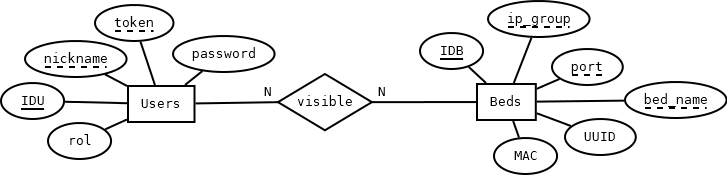
\includegraphics[width=\textwidth]{img/entidad-relacion.png}
	\caption{Diagrama entidad-relación}
	\label{fig:erDia}
\end{figure}

De este diagrama generamos el diagrama relacional (figura~\ref{fig:relational}) en el que se especifican las tablas que se usarán en el producto final.

\begin{figure}
	\centering
	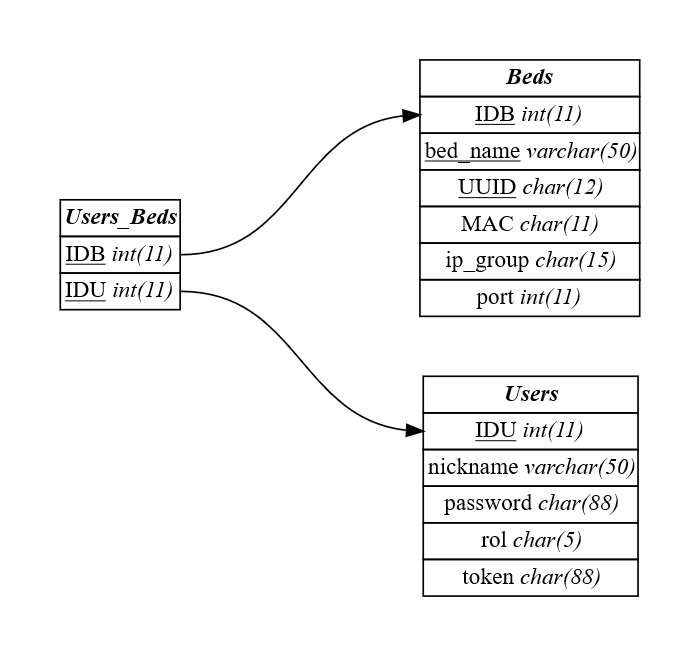
\includegraphics[width=0.5\textwidth]{relational}
	\caption{Diagrama relacional}
	\label{fig:relational}
\end{figure}


\section{Diseño procedimental}

\section{Diseño arquitectónico}

\section{Diseño de interfaces}

Las interfaces se han diseñado teniendo en cuenta la usabilidad de la misma así como un diseño simple que permitiese que fuese más intuitiva con una curva de aprendizaje leve. Se ha tenido en cuenta también que la interfaz sea adaptable a una gran variedad de pantallas teniendo en cuenta que, al ser una aplicación web, el uso de la misma puede ser en multitud de dispositivos diferentes.

%TODO: Hacer test de usabilidad con personal sanitario

Los primeros prototipos fueron realizados sobre el caso de uso especificado en la tabla~\ref{tabla:tablaCU22}, tanto para escritorio (imagen~\ref{fig:proto-desk}) como para móvil (imagen~\ref{fig:proto-mob}).

\begin{figure}[h]
	\centering
	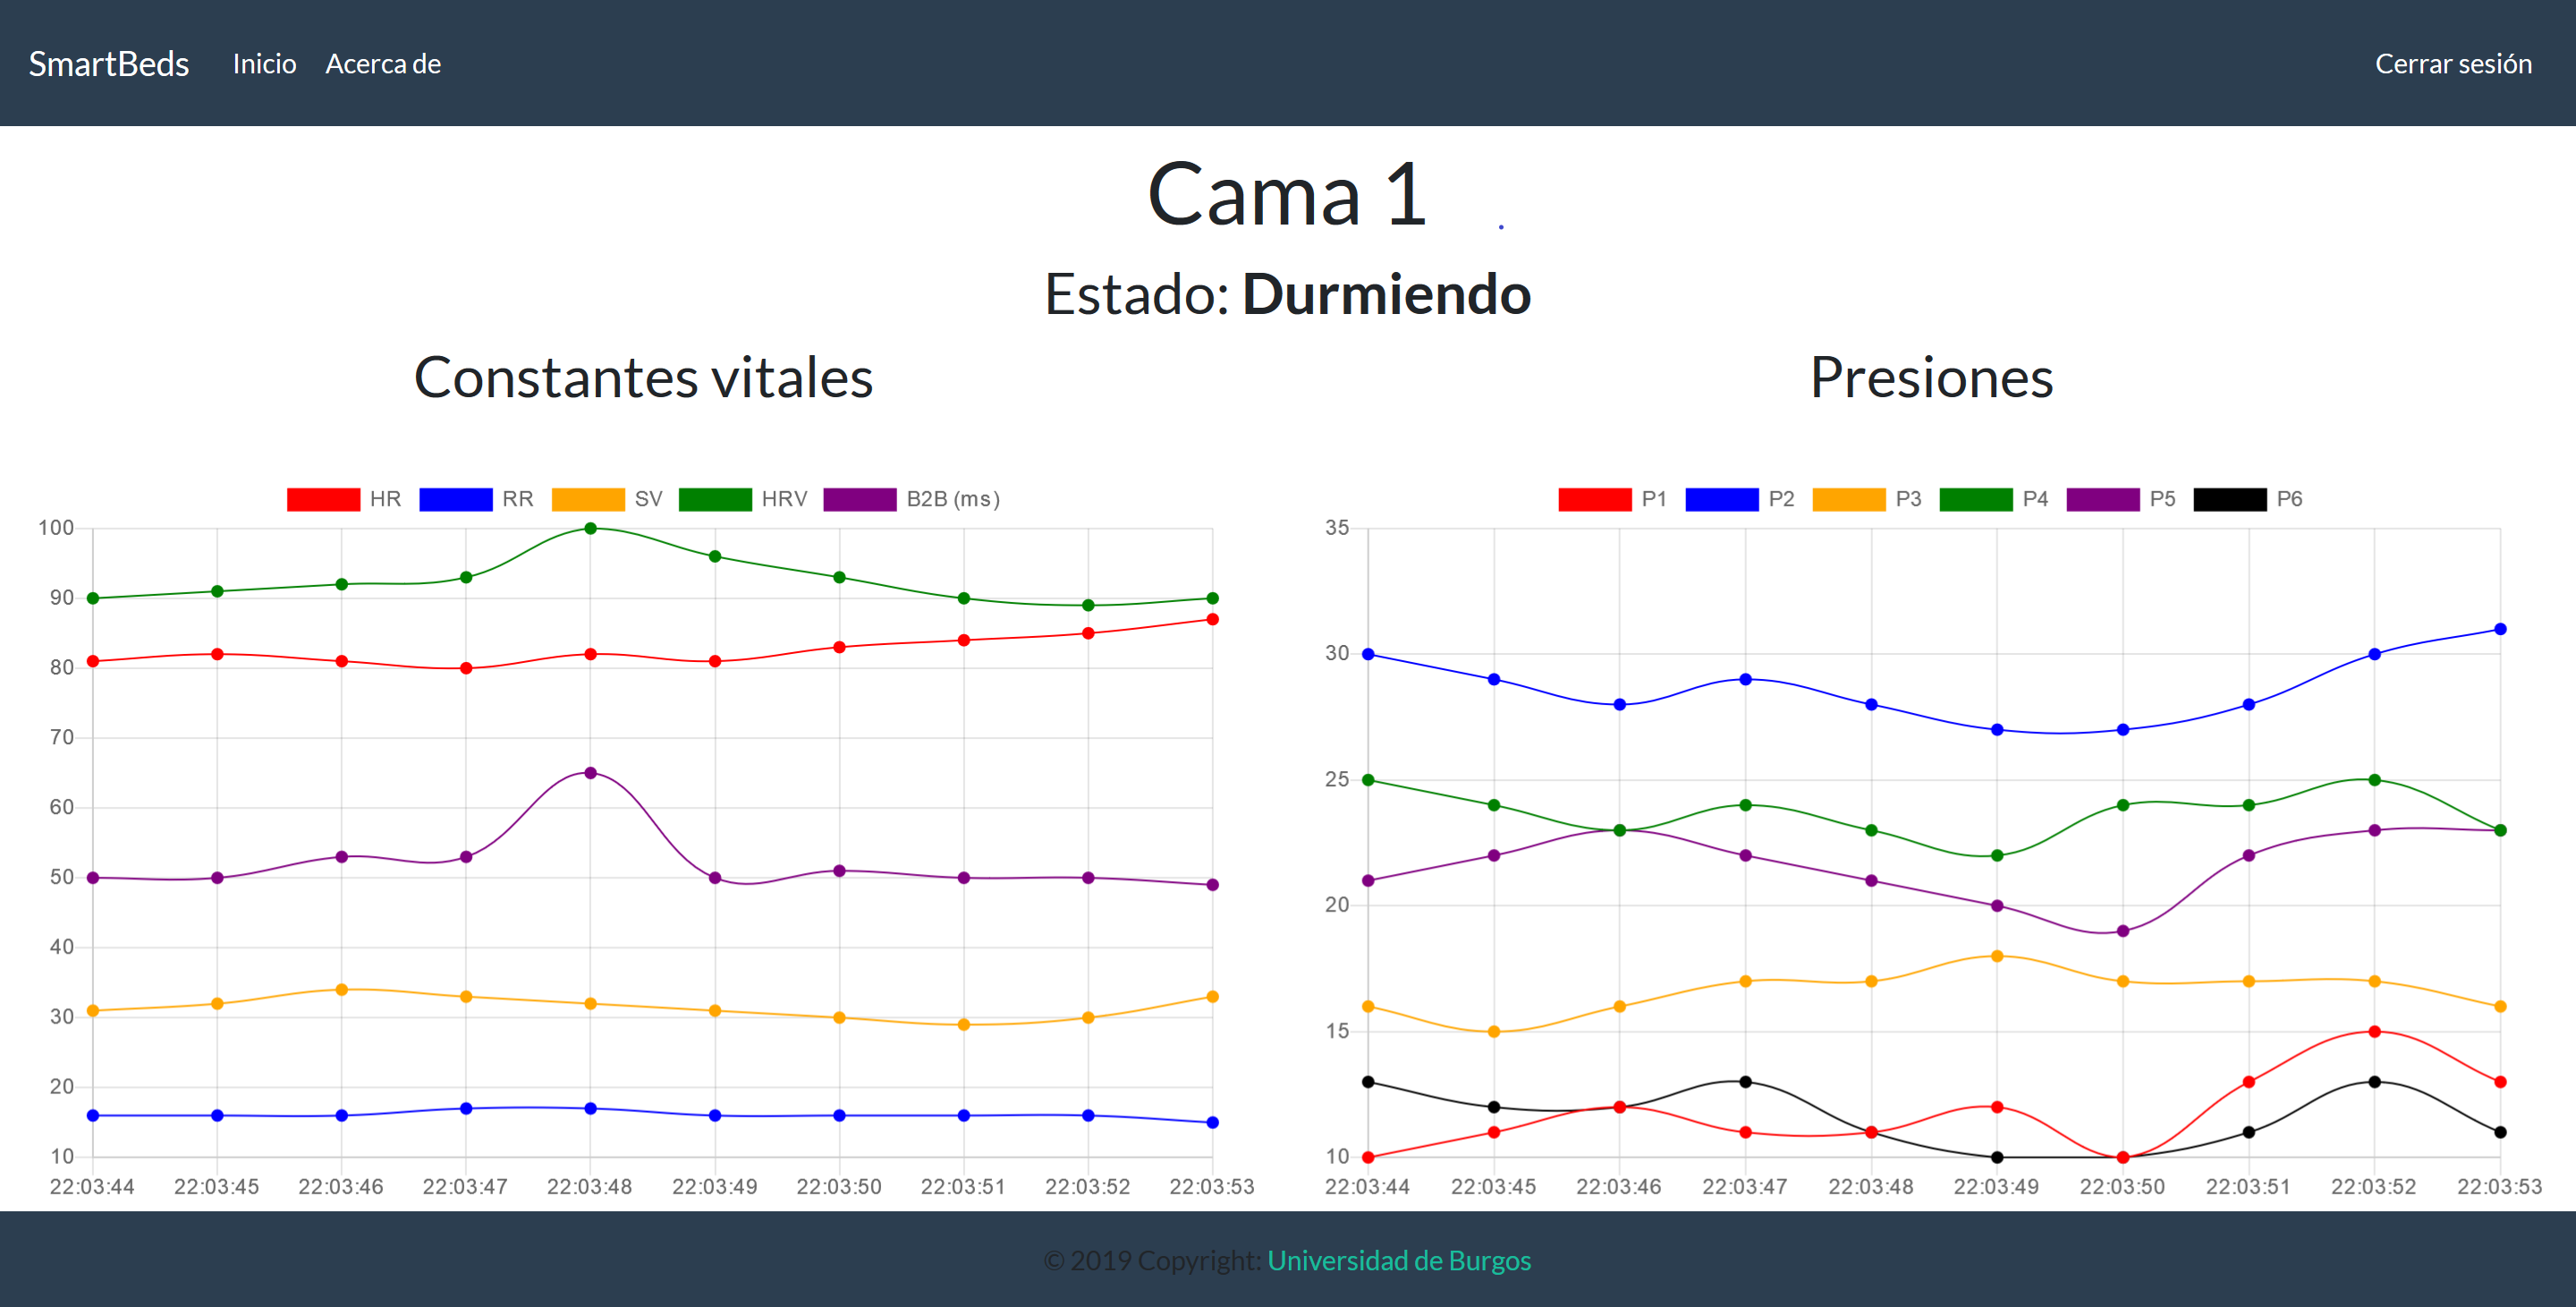
\includegraphics[width=\textwidth]{prot-desktop}
	\caption{Prototipo para escritorio}
	\label{fig:proto-desk}
\end{figure}

\begin{figure}[h]
	\centering
	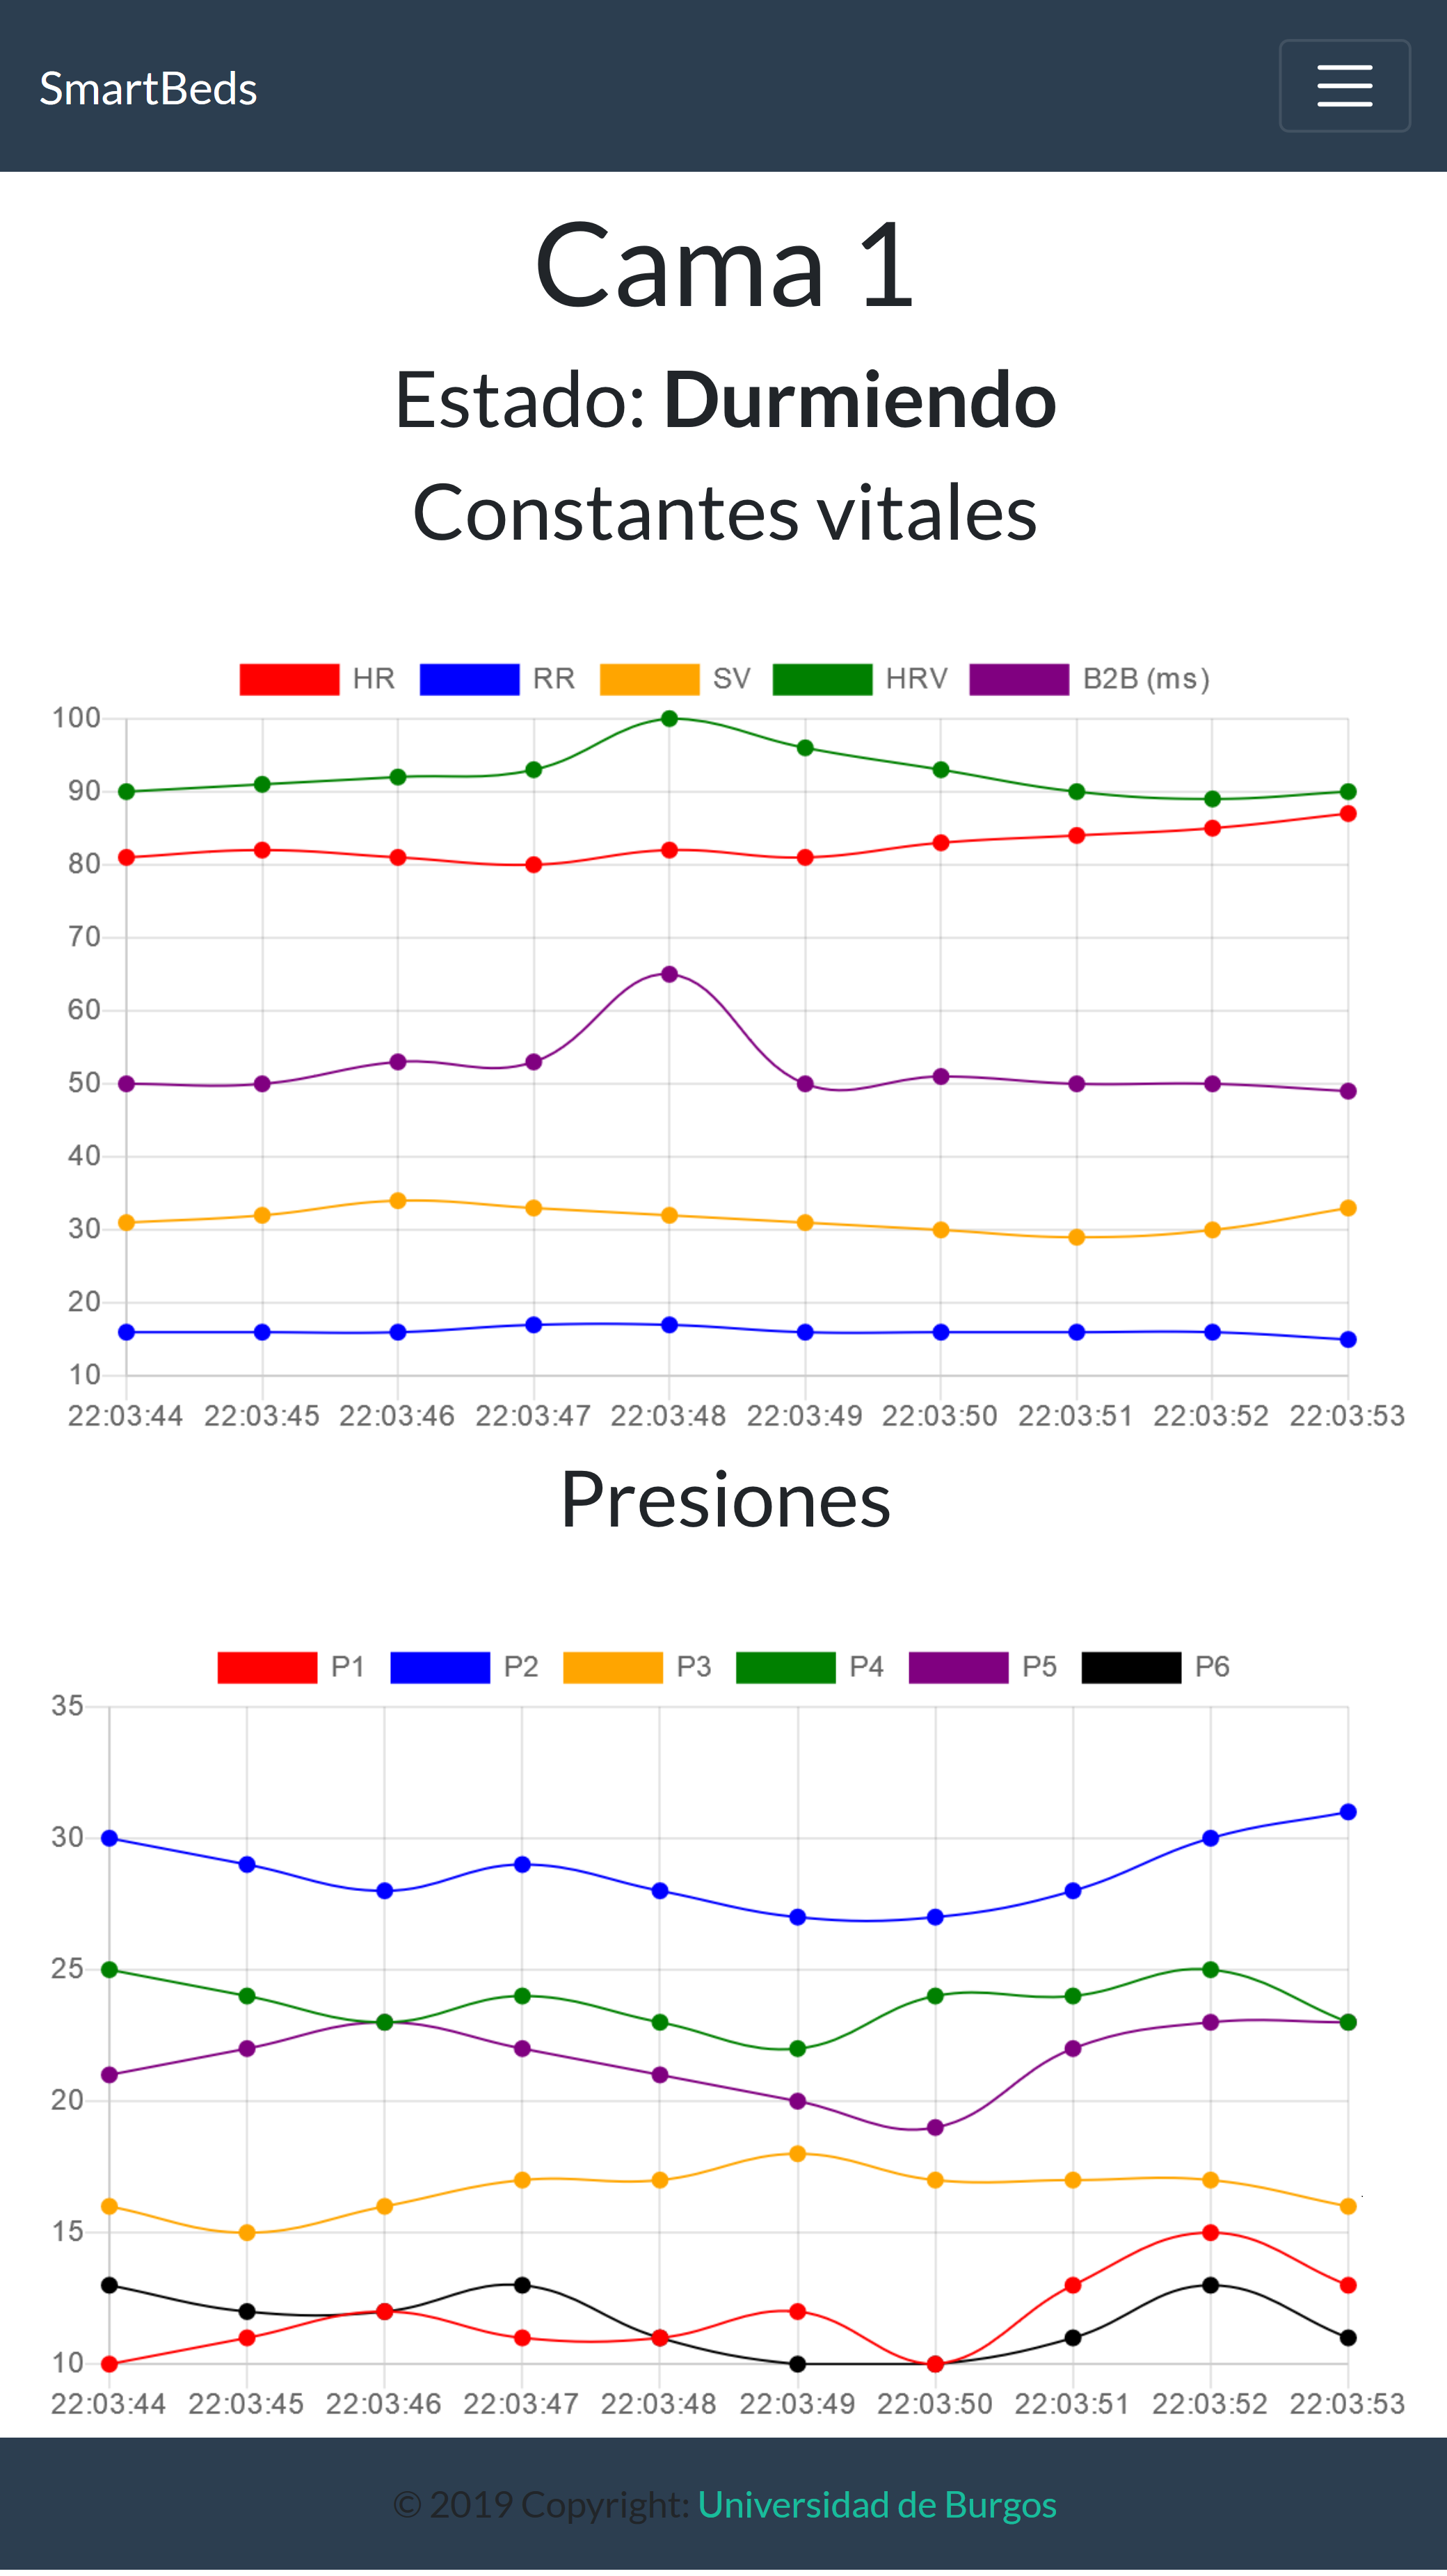
\includegraphics[width=0.45\textwidth]{prot-mobile}
	\caption{Prototipo para móvil}
	\label{fig:proto-mob}
\end{figure}
